\section{Architecture}
\label{SEC:architecture}

\begin{figure}
  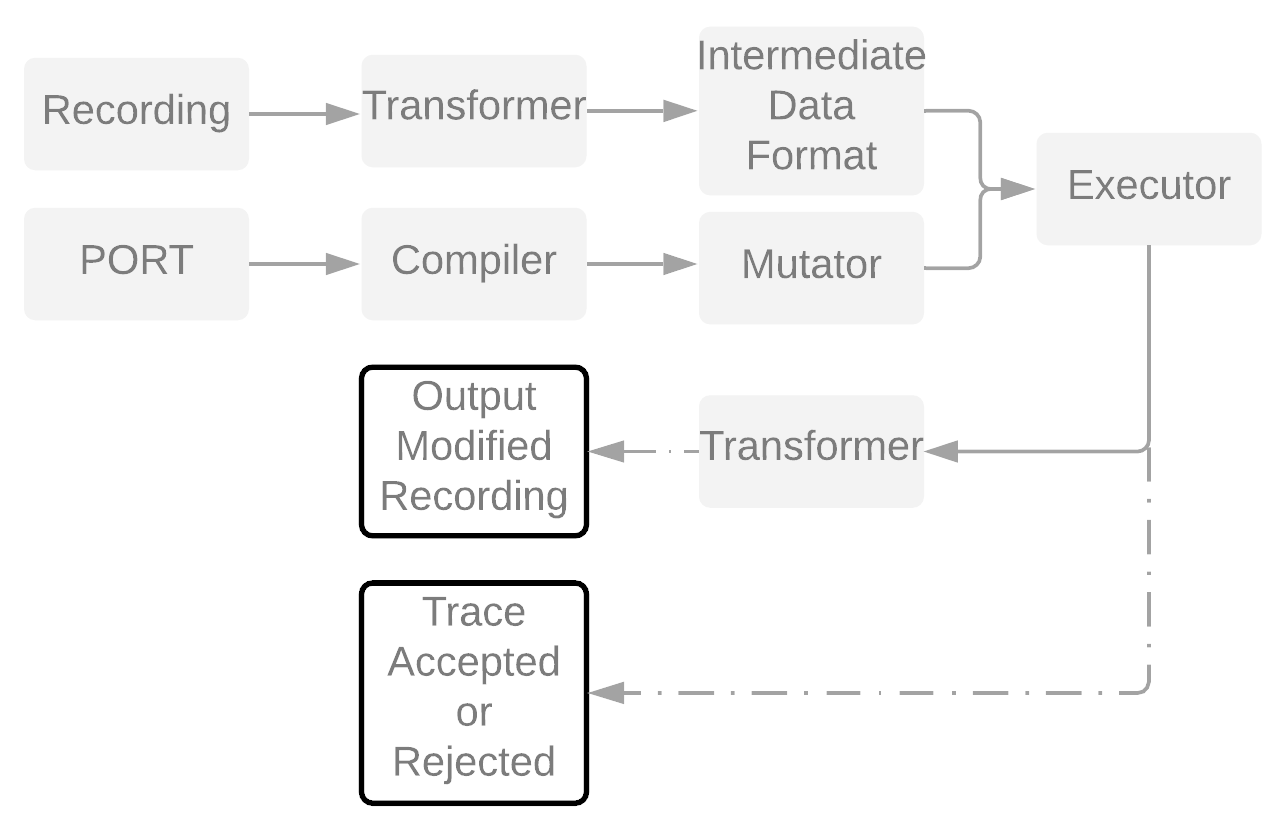
\includegraphics[scale=.08, frame]{images/architecture}
  \caption{The CSLang compiler produces a transducer that operates over a
  generic intermediate representation of the contents of a given trace.}
  \label{fig:architecture}
\end{figure}


The SEA technique's power comes from its ability to capture and encode
anomalies so they can be repeatedly employed to test applications.  But, as
previous work discussed, taking advantage of this feature can be
challenging.  Based on these qualities, we reasoned the capture process
was a good candidate for our improvement efforts.
As a first step, we examined the encoded anomalies used in the
earlier SEA work and found several deficiencies.
They were
long (in terms of lines of code),
difficult to read and maintain,
and tightly coupled to the implementation details of system calls.
We decided to address each of these concerns by developing a new
programming language, CSLang.  Our goal with CSLang was to provide a way to
describe anomalies that was concise, easy to understand, and generic enough
that it could support many message formats.

While the development of CSLang
is the star of the show,
it is important to first understand
several new components
that form the language's foundation.
At the core of our efforts is
a new model for recognizing and transforming streams of messages.  Our
model is based on a finite-state transducer and builds upon the earlier SEA
work's success at describing simulation opportunities using deterministic
finite automata.  We chose the transducer as our foundation so that
recognition and transformation of streams could be done at the same time.
This model is generated by compiling a CSLang anomaly description.

The model does not serve much purpose without a stream of messages to
operate on.
This stream is provided by our second component,
the message format adaptor,
which takes
stream of messages in their original representation and converts
them into a format that a CSLang transducer can consume. This conversion process
captures the identifying information and parameters of each message in the
input stream and stores them in CSLang's Intermediate Data Format (IDF).
Operating on this generic intermediate format means CSLang transducers are
not dependent on a specific message format.

%This is important because it
%breaks the system-call dependence of the previous SEA work allowing

%% which helps us achieve our third goal and
A final component, known as the CSLang executor,
receives both the transducer and the converted message stream.
This program is responsible for passing each message of the stream
to the transducer
so that it may advance its internal state and
produce the appropriate output.
In this case, output comes in the form of modifications to the IDF stream itself.
If the transducer is
ends in an accepting state, the stream of messages has
been modified to include an anomaly and will be output in its original
representation.  If the automaton is not in an accepting state, the stream
did not contain an opportunity to simulate the described anomaly.

<Something Something Something how simulation works goes here?>

%\begin{itemize}
%  \item{Language describing anomalies}
%  \item{Formal model of transducer that can implement anomalies}
%  \item{Tool to compile description into said formal transducer}
%  \item{Format-agnostic intermediate data structure (IDS) over which transducer
%  operates}
%  \item{Translation layer for converting to and from concrete data into IDS}
%\end{itemize}

